%%%%%%%%%%%%%%%%%%%%%%%%%%%%%%%%%%%%%%%%%
% Thin Sectioned Essay
% LaTeX Template
% Version 1.0 (3/8/13)
%
% This template has been downloaded from:
% http://www.LaTeXTemplates.com
%
% Original Author:
% Nicolas Diaz (nsdiaz@uc.cl) with extensive modifications by:
% Vel (vel@latextemplates.com)
%
% License:
% CC BY-NC-SA 3.0 (http://creativecommons.org/licenses/by-nc-sa/3.0/)
%
%%%%%%%%%%%%%%%%%%%%%%%%%%%%%%%%%%%%%%%%%

%----------------------------------------------------------------------------------------
%	PACKAGES AND OTHER DOCUMENT CONFIGURATIONS
%----------------------------------------------------------------------------------------

\documentclass[a4paper, 11pt]{article} % Font size (can be 10pt, 11pt or 12pt) and paper size (remove a4paper for US letter paper)

\usepackage[protrusion=true,expansion=true]{microtype} % Better typography
\usepackage{graphicx} % Required for including pictures
\usepackage{wrapfig} % Allows in-line images

\usepackage{mathpazo} % Use the Palatino font
\usepackage[T1]{fontenc} % Required for accented characters
%\usepackage[backend=bibtex,style=verbose-trad2]{biblatex}
\usepackage{hyperref}
\usepackage{longtable}
\usepackage{array}
\usepackage{multirow}
\usepackage[utf8]{inputenc}
\usepackage{subcaption}
\usepackage[font=small]{caption}

\linespread{1.05} % Change line spacing here, Palatino benefits from a slight increase by default

\makeatletter
\renewcommand\@biblabel[1]{\textbf{#1.}} % Change the square brackets for each bibliography item from '[1]' to '1.'
\renewcommand{\@listI}{\itemsep=0pt} % Reduce the space between items in the itemize and enumerate environments and the bibliography

\renewcommand{\maketitle}{ % Customize the title - do not edit title and author name here, see the TITLE block below
\begin{flushright} % Right align
{\LARGE\@title} % Increase the font size of the title

\vspace{50pt} % Some vertical space between the title and author name

{\large\@author} % Author name
\\\@date % Date

\vspace{40pt} % Some vertical space between the author block and abstract
\end{flushright}
}

%----------------------------------------------------------------------------------------
%	TITLE
%----------------------------------------------------------------------------------------

\title{\textbf{Slimme Cruise Control}\\ % Title
implementatie onderzoek} % Subtitle

\author{\textsc{Rowan Bolding \\
	studentnummer: 500757732 \\
	e-mail: Rowan.Bolding@hva.nl} % Author
\\{\textit{Amsterdam University of Applied Sciences\\ 
Innovatielab}}} % Institution

\date{17 september, 2019} % Date

%----------------------------------------------------------------------------------------
\bibliographystyle{IEEEtran}
\begin{document}
\captionsetup[figure]{labelfont={bf},name={Fig},labelsep=period}
\captionsetup{justification=centering}
\hypersetup{hidelinks=true}
\maketitle % Print the title section

%----------------------------------------------------------------------------------------
%	ABSTRACT AND KEYWORDS
%----------------------------------------------------------------------------------------

%\renewcommand{\abstractname}{Summary} % Uncomment to change the name of the abstract to something else


\vspace{10pt} % Some vertical space between the abstract and first section

%----------------------------------------------------------------------------------------
%	ESSAY BODY
%----------------------------------------------------------------------------------------
\newpage

\tableofcontents

\newpage
%----------------------------------------------------------------------------------------
\section{inleiding}
Clean Mobility is een project van de HvA waarbij er wordt gewerkt aan de ontwikkeling van de volgende 3 voertuigen:
\begin{description}
	\item$\bullet${ \textbf{De Solar Boat:}}\\
		dit is een boot die op zonne-energie vaart. Op het “dek” van deze boot liggen zonnepanelen.
	\item$\bullet${ \textbf{De H2A:}}\\
		dit is een auto die op waterstof rijdt. Bij de ontwikkeling van deze auto ligt de focus op het zo efficiënt/energiezuinig mogelijk rijden, zo heeft deze bijvoorbeeld de vorm van een regendruppel.
	\item$\bullet${ \textbf{De EVA:}}\\
		Dit is een auto die op elektriciteit rijdt en kan autonoom rijden. Hoewel ook bij deze auto de focus op efficiëntie/energiezuinigheid ligt, is het ook de bedoeling dat deze auto zo veel mogelijk wordt benaderd als een “gewone auto”.
	\item$\bullet${ \textbf{De SPIRIT:}}\\
		Dit is een auto die tegenwind gebruikt als energiebron. De windenergie wordt opgevangen door een rotor, waarmee het in bewegingsenergie wordt omgezet wat er weer voor zorgt dat de auto vooruit rijd.
	
\end{description}
Het doel bij de H2A en de EVA is dat ze gaan meedoen aan de Shell eco-marathon. Hierbij worden er races gedaan tegen andere universiteiten en hogescholen van over de hele wereld. Bij deze races moet het voertuig binnen een bepaalde tijd een aantal rondes hebben gereden op een zo efficiënt mogelijke manier. Verder doet de EVA ook nog mee aan een wedstrijd die zich richt op het autonoom rijden.  Omdat de focus bij de races ligt op zuinigheid, is de rijstrategie een belangrijk onderdeel bij Clean Mobility. De rijstrategie berekend per deel van de racebaan uit wat de meest efficiënte snelheid is op te rijden, om zo de race zo zuinig efficiënt mogelijk uit te rijden. Het is echter voor de bestuurders van deze voertuigen vaak lastig om per deel van de racebaan op de meest efficiënte snelheid te blijven rijden, dit valt te wijten aan verschillende omstandigheden. Zo kan de communicatie van de bestuurder met het team aan de kant slecht zijn, de bestuurder kan het simpelweg vergeten zijn, de bestuurder beschikt simpelweg niet over de kwaliteiten om de auto op een constante snelheid te houden, de snelheid die de bestuurder krijgt doorgegeven via het dashboard klopt niet, etc… \\
Kortom: het voertuig daadwerkelijk op elk deel van de racebaan de meest efficiënte snelheid te laten rijden is te afhankelijk van menselijke fouten.
%----------------------------------------------------------------------------------------
\section{Global Position System (GPS)}
De huidige GPS modules (de Sparkfun met de Venus638FLPx chip en de NavSpark met de Venus828F chip) hebben een absolute nauwkeurigheid 2,5m CEP. Dit houd in dat je daadwerkelijke positie binnen een straal van 2,5 meter zit t.o.v. de verkregen positie uit de GPS module.

\begin{figure}[h!]
	\centering
%	\hspace*{-2cm}
	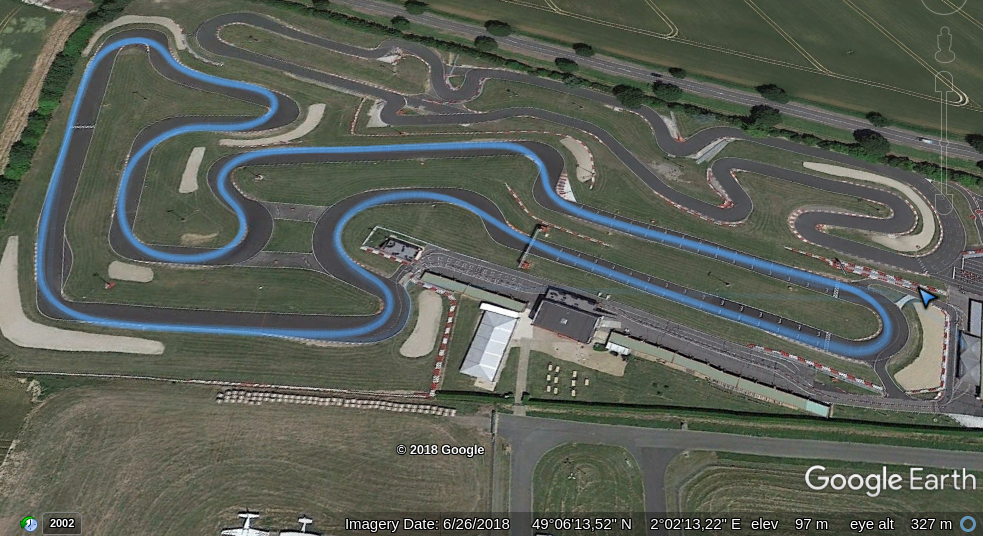
\includegraphics[width=15cm]{afbeeldingen/Parijstest.png}
	\caption{De endurance-rit van de EVA tijdens de Shell eco-marathon in Parijs (2018)}
\end{figure}

\begin{figure}[h!]
	\centering
	%	\hspace*{-2cm}
	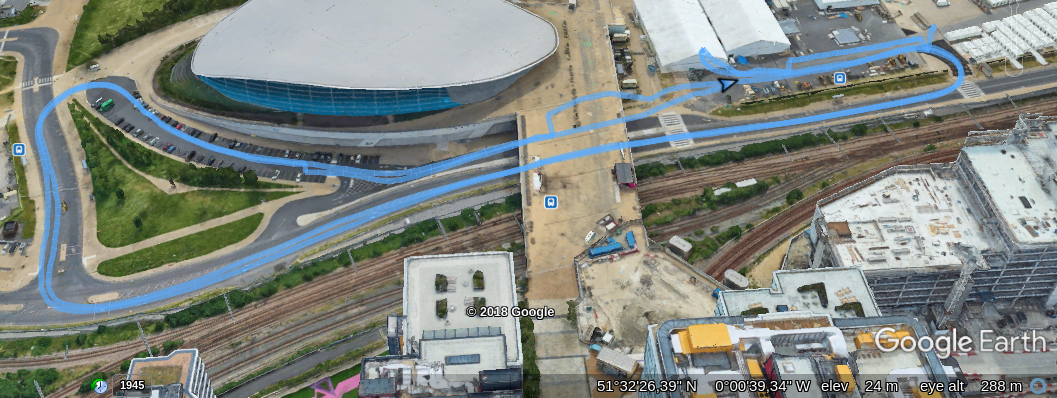
\includegraphics[width=15cm]{afbeeldingen/Londontest.png}
	\caption{Een score-rit van de H2A tijdens de Shell eco-marathon in London (2018)}
\end{figure}
\newpage
In figuur 1 en 2 zijn de 2 verschillende races te zien, in figuur 1 de EVA in Parijs en in figuur 2 de H2A in London. Een belangrijk verschil tussen deze twee races is dat de race in Parijs werd gereden in een erg open omgeving zonder al te veel gebouwen en voornamelijk weilanden om de baan heen, terwijl de race in London redelijk in het centrum van London werd gereden (naast het olympisch stadion) omringd door gebouwen. Dit heeft als gevolg dat het GPS-signaal tijdens de race in London veel rommeliger was dan tijdens de race in Parijs. GPS vereist een directe line of sight, de nauwkeurigheid van GPS zal er onder lijden wanneer dit niet zo is wegens signaal reflectie en een zwakker signaal in het algemeen. Wanneer de GPS ontvanger zich bevindt in een “gesloten” ruimte, zoals een stad met veel hoge gebouwen of in een bos, kan de GPS ontvanger minder satellieten zien en zijn de satellieten die hij ziet minder verspreid. Hierdoor kan je locatie niet berekend worden vanuit meerdere richtingen, maar zitten de satellieten die gebruikt worden voor het berekenen van je locatie geclusterd in een klein gebied[1]. De omgeving van het voertuig heeft dus erg veel invloed op de sterkte van het GPS signaal en de nauwkeurigheid van de informatie die ontvangen wordt.
\subsection{RTK GPS}
Over het algemeen is GPS zelfs in de meest ideale omgevingen niet nauwkeurig genoeg om leidend te zijn voor het bepalen van de snelheid op een veilige manier. Een GPS-toepassing die veel meer nauwkeurigheid oplevert is RTK. RTK staat voor Real Time Kinematic en maakt gebruik van een basis station. Met RTK worden in het basis station en in een mobiele ontvanger faseverschillen gemeten tussen een signaal dat uit de satellieten binnenkomt en een identiek signaal wat door de ontvangers zelf gegenereerd wordt. Met een geheel aantal golflengten en de faseverschillen wordt door middel van de afstanden naar de satellieten een basislijn berekend tussen de twee ontvangers. De basislijn vormt een relatieve positie van de mobiele ontvanger t.o.v. het basis station. Doordat de positie van de basis station vooraf nauwkeurig is ingemeten krijg je een nauwkeurige positie van de mobiele ontvanger [2]. In figuur 3 op de volgende pagina is het verschil tussen RTK GPS en de gewone GPS goed te zien.
\newpage
\begin{figure}[h!]
	\centering
	%	\hspace*{-2cm}
	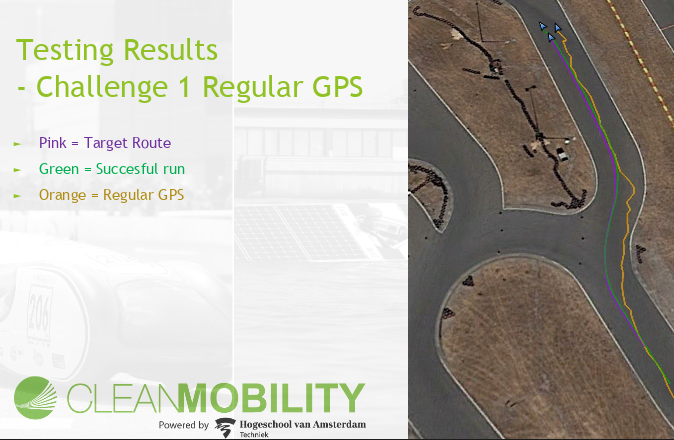
\includegraphics[width=12cm]{afbeeldingen/RTKvsNorm.PNG}
	\caption{RTK GPS (groen) naast gewone GPS (oranje) [3]}
\end{figure}
RTK GPS kan een nauwkeurigheid hebben tot op tientallen centimeters CEP, wat tegenover de 2,5m CEP van gewone GPS toepassingen een flinke verbetering is. Om RTK GPS te laten werken moeten er minimaal 6 satellieten te zien zijn. In een dicht bebouwde omgeving is dus ook RTK GPS niet betrouwbaar genoeg om het leidend te laten zijn over het bepalen van de snelheid van het voertuig [2]. Voor het realiseren van een betrouwbare SCC kan er dus niet alleen worden uitgegaan van GPS data.
%----------------------------------------------------------------------------------------
\section{Beweging van het voertuig zelf.}
Een accelerometer meet de fysieke versnelling die een object ervaart. In stilstand(of tijdens een beweging met een constante snelheid) op het aardoppervlak zal de accelerometer de valversnelling (of gravitatieveld sterkte) van 1g of \begin{math}	9,81m/s^{2} \end{math} teruggeven, ongeacht de oriëntatie van de sensor. Om de versnelling van een beweging ten opzichte van de aarde te verkrijgen zal de offset van de zwaartekracht worden afgetrokken.
\begin{center}
	[4]\\
	\begin{math}
	a_{beweging} = a_{totaal} - a_{zwaartekracht}
	\end{math}
\end{center}
De versnelling is verspreid over deze 3 assen, wat betekent dat in stilstand (of bij de beweging met een constante snelheid) de resulterende vector van deze 3 assen loodrecht op de aarde staat en een waarde heeft van 1g ongeacht de oriëntatie van de sensor.
\newpage
\begin{figure}[h!]
	\centering
	\hspace*{-2cm}
	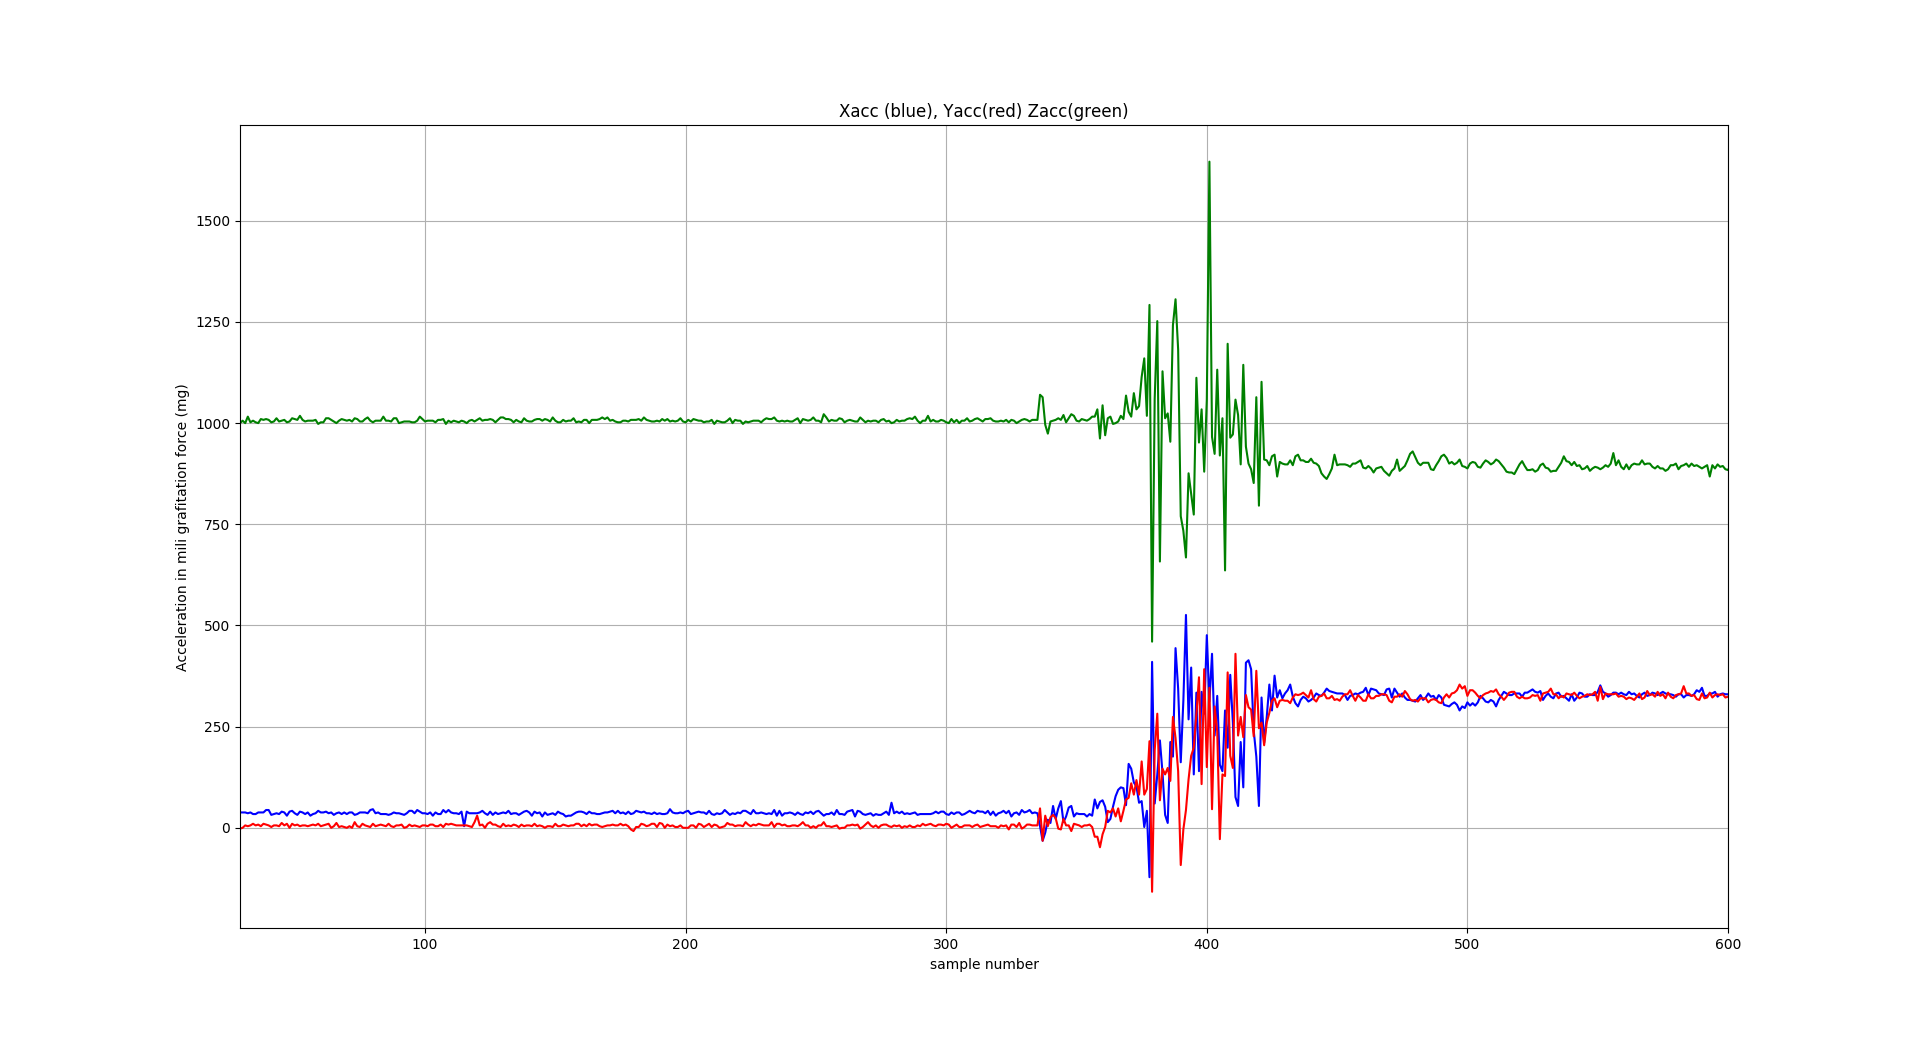
\includegraphics[width=16cm]{afbeeldingen/rawAcc.png}
	\caption{Rauwe data uit de sensor tijdens test met beweging in 1 richting (blauw: x-as, rood: y-as \& groen: z-as)}
\end{figure}
In figuur 4 is de rauwe data van de accelerometer te zien tijdens een test waarbij de sensor kort in een bepaalde richting wordt bewogen en tijdens deze beweging een beetje van oriëntatie veranderd. Op het moment dat lijnen over van 3 assen heftig beginnen te fluctueren, is er sprake van een versnelling/afremming. Op het moment dat de lijnen zijn gestopt met heftig fluctueren is de sensor of in beweging met een constante snelheid, of staat de sensor stil. In dit geval is het vooraf al bekend dat de sensor stil staat aan het eind van de test. Na de beweging gaan zijn de gemeten versnellingen van de 3 assen niet meer rond de zelfde waarde als voor de beweging, dit komt door de verandering van oriëntatie tijdens de beweging. Deze data oogt nog er rommelig, dit valt toe te wijden aan ruis. ook is de offset van de zwaartekracht terug te vinden in deze data. Om een goed beeld te krijgen van de daadwerkelijke versnelling/afremming van de sensor zal de data dus gefilterd moeten worden en de offset van de zwaartekracht moeten worden afgetrokken. Wanneer dit is gebeurd kan de data van de accelerometer verwerkt worden. Door de versnelling te integreren over tijd, wordt de snelheid van de sensor verkregen. Waar de versnelling de verandering van de snelheid over tijd is, is de snelheid de verandering van verplaatsing over tijd. Door de snelheid te integreren (en dus eigenlijk de versnelling dubbel te integreren) zou in theorie de verplaatsing uit de versnellingsdata te verkrijgen moeten zijn.
\newpage
\begin{figure}[h!]
	\centering
	\hspace*{-2cm}
	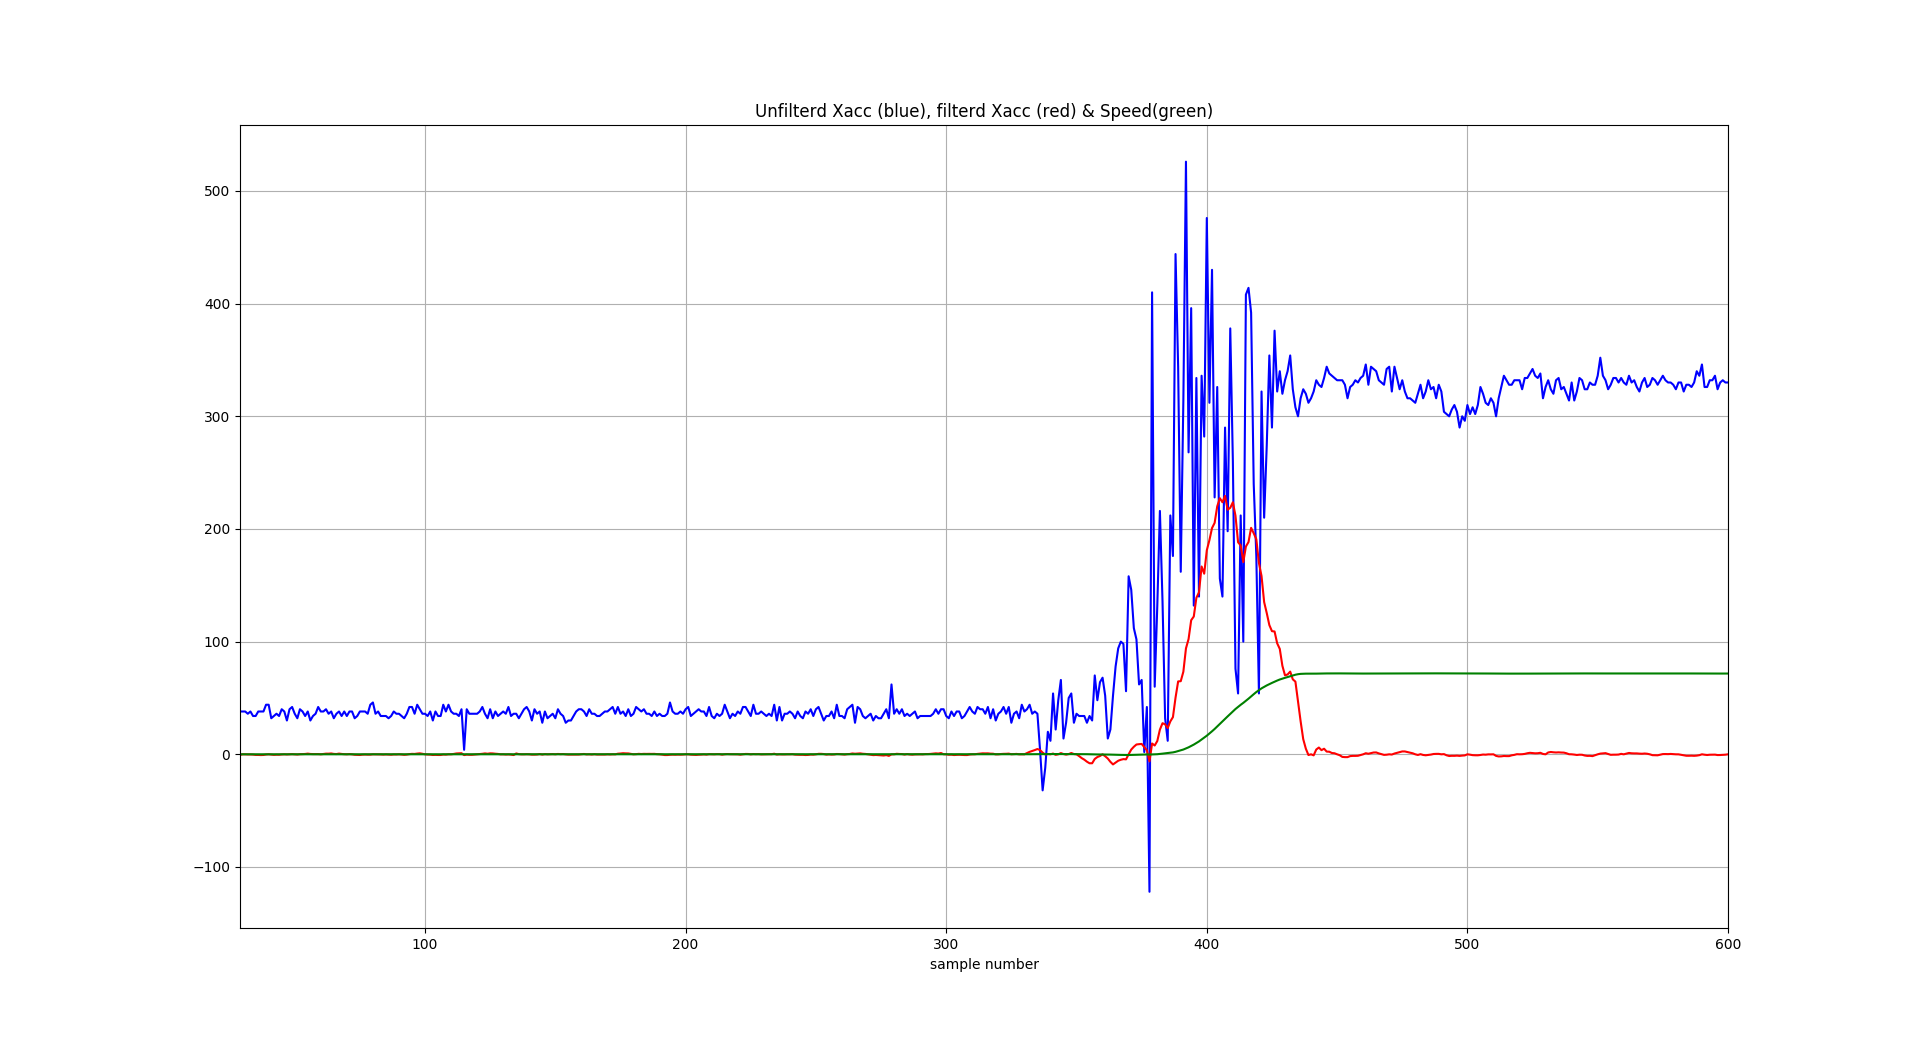
\includegraphics[width=16cm]{afbeeldingen/XasPlot.png}
	\caption{Data over de x-as van de sensor (blauw: ongefilterd, rood: gefilterd \& groen: snelheid)}
\end{figure}
Voor het gemak is er in figuur 14 ervoor gekozen om alleen de data over de x-as van de sensor te weergeven (zie omschrijving figuur 14). Te zien is dat de snelheid op een gegeven moment een offset krijgt, ter gevolge van de verandering in oriëntatie tijdens de beweging. Door de verandering van de oriëntatie is de zwaartekracht weer op een andere manier verdeeld over de sensor, waarbij de verdeling onbekend is. Het is alleen mogelijk om tijdens een beweging met een constante snelheid of in stilstand te bepalen hoe de zwaartekracht verdeeld is over de 3 assen. Dit zorgt er voor dat wanneer de oriëntatie veranderd middenin een versnellende beweging, de zwaartekracht niet meer correct gecorrigeerd kan worden tot en er sprake is van beweging met een constante snelheid of geen beweging (stil staan). Deze offset zorgt er voor dat bij het eerste integraal de snelheid nooit terug op 0 komt ook al staat de sensor stil. Omdat de snelheid nooit terug komt op 0 bij stilstand, komt voort uit de data dat de sensor nog steeds in beweging is terwijl dit niet zo is. Wanneer de oriëntatie van de sensor bekend, kan ook de verdeling van de zwaartekracht over de 3 assen tijdens een versnellende/afremmende beweging bepaald kunnen worden.
\newpage
\subsection{Gyroscoop}
%----------------------------------------------------------------------------------------
%	BIBLIOGRAPHY
%----------------------------------------------------------------------------------------
\newpage
\begin{thebibliography}{9}
	\bibitem{Openstreetmap}
	openstreetmap,
	29-07-2019 [Bekeken in september 2019],
	[Online],
	Beschikbaar: \url{https://wiki.openstreetmap.org/wiki/Accuracy_of_GPS_data}

	\bibitem{Edge documentatie}
	A. Iyiade,
	University of Plymouth,
	09-01-2009 [Bekeken in september 2019],
	[Online],
	"Real Time Kinematic GPS in an Urban Canyon Environment",
	Beschikbaar: \url{https://www.geospatialworld.net/article/real-time-kinematic-gps-in-an-urban-canyon-environment/}

	\bibitem{Thierry}
	Thierry Ligeon,
	Amsterdam University of Applied Sciences,
	2016 [Bekeken in maart 2019],
	[Presentatie]
	
	\bibitem{Openstreetmap}
	Ryan Goodrich,
	LiveScience,
	01-10-2013 [Bekeken in september 2019],
	[Online],
	"Accelerometers: What They Are \& How They Work",
	Beschikbaar: \url{https://www.livescience.com/40102-accelerometers.html}
\end{thebibliography}
%----------------------------------------------------------------------------------------
\end{document}
